\documentclass[notitlepage,a4paper,12pt,norsk]{IMFeksamen}
\usepackage[utf8]{inputenc}
\emnekode{TMA4110}
\emnenavn{Matematikk 3 -- EKSEMPEL~1}
\runninghead{TMA4110 -- Eksamen høsten 2018 -- EKSEMPEL~1 -- Løsning}
\usepackage[T1]{fontenc}
\usepackage{lmodern,amsmath,amssymb,amsfonts}
\usepackage{mathrsfs}
\usepackage{systeme}
\usepackage{tikz}
\usepackage{pgfornament}

\newcommand{\N}{\mathbb{N}}
\newcommand{\Z}{\mathbb{Z}}
\newcommand{\Q}{\mathbb{Q}}
\newcommand{\R}{\mathbb{R}}
\newcommand{\C}{\mathbb{C}}

\newcommand{\M}{\mathcal{M}} % vektorrom av matriser
\newcommand{\Cf}{\mathcal{C}} % vektorrom av kontinuerlige funksjoner
\renewcommand{\P}{\mathcal{P}} % vektorrom av polynomer
\newcommand{\B}{\mathscr{B}} % basis

\renewcommand{\Im}{\operatorname{Im}}
\renewcommand{\Re}{\operatorname{Re}}

\newcommand{\abs}[1]{|#1|}
\newcommand{\intersect}{\cap}
\newcommand{\union}{\cup}
\newcommand{\fcomp}{\circ}
\newcommand{\iso}{\cong}

\newcommand{\roweq}{\sim}
\DeclareMathOperator{\Sp}{Sp}
\DeclareMathOperator{\Null}{Null}
\DeclareMathOperator{\Col}{Col}
\DeclareMathOperator{\Row}{Row}
\DeclareMathOperator{\rank}{rank}
\DeclareMathOperator{\im}{im}
\DeclareMathOperator{\id}{id}
\DeclareMathOperator{\Hom}{Hom}
\newcommand{\tr}{^\top}
\newcommand{\koord}[2]{[\,{#1}\,]_{#2}} % koordinater mhp basis

\newcommand{\V}[1]{\mathbf{#1}}
\newcommand{\vv}[2]{\begin{bmatrix} #1 \\ #2 \end{bmatrix}}
\newcommand{\vvS}[2]{\left[ \begin{smallmatrix} #1 \\ #2 \end{smallmatrix} \right]}
\newcommand{\vvv}[3]{\begin{bmatrix} #1 \\ #2 \\ #3 \end{bmatrix}}
\newcommand{\vvvv}[4]{\begin{bmatrix} #1 \\ #2 \\ #3 \\ #4 \end{bmatrix}}
\newcommand{\vvvvv}[5]{\begin{bmatrix} #1 \\ #2 \\ #3 \\ #4 \\ #5 \end{bmatrix}}
\newcommand{\vn}[2]{\vvvv{#1_1}{#1_2}{\vdots}{#1_#2}}

\newcommand{\e}{\V{e}}
\renewcommand{\u}{\V{u}}
\renewcommand{\v}{\V{v}}
\newcommand{\w}{\V{w}}
\renewcommand{\b}{\V{b}}
\newcommand{\x}{\V{x}}
\newcommand{\0}{\V{0}}

\newenvironment{amatrix}[1]{% "augmented matrix"
  \left[\begin{array}{*{#1}{c}|c}
}{%
  \end{array}\right]
}

\newcommand{\oppgslutt}{
\begin{center}
\pgfornament[width=6cm]{88}
\end{center}
}
\newenvironment{losning}{\begin{oppgave}}{\oppgslutt\end{oppgave}}


\begin{document}


\begin{losning}
Totalmatrise:
$
\begin{bmatrix}
0 & 2 & 4 &   2 & 6 \\
2 & 1 & 2 & -13 & 3 \\
1 & 3 & 6 &  -4 & 9
\end{bmatrix}
$.
Vi radreduserer matrisen:
\begin{align*}
\begin{bmatrix}
0 & 2 & 4 &   2 & 6 \\
2 & 1 & 2 & -13 & 3 \\
1 & 3 & 6 &  -4 & 9
\end{bmatrix}
&\sim 
\begin{bmatrix}
1 & 3 & 6 &  -4 & 9 \\
2 & 1 & 2 & -13 & 3 \\
0 & 2 & 4 &   2 & 6
\end{bmatrix}
\sim
\begin{bmatrix}
1 & 3 & 6 &  -4 & 9 \\
0 & -5 & -10 & -5 & -15 \\
0 & 2 & 4 &   2 & 6
\end{bmatrix}\\
&\sim 
\begin{bmatrix}
1 & 3 & 6 &  -4 & 9 \\
0 & 1 & 2 & 1 & 3 \\
0 & 2 & 4 &   2 & 6
\end{bmatrix}
\sim
\begin{bmatrix}
1 & 3 & 6 &  -4 & 9 \\
0 & 1 & 2 & 1 & 3 \\
0 & 1 & 2 & 1 & 3
\end{bmatrix}\\
&\sim 
\begin{bmatrix}
1 & 3 & 6 &  -4 & 9 \\
0 & 1 & 2 & 1 & 3 \\
0 & 0 & 0 &  0 & 0
\end{bmatrix}
\sim
\begin{bmatrix}
1 & 0 & 0 &  -7 & 0 \\
0 & 1 & 2 & 1 & 3 \\
0 & 0 & 0 &  0 & 0
\end{bmatrix}.
\end{align*}
Dette gir likningene 
$$x_1-7x_4=0$$
og $$x_2+2x_3+x_4=3.$$
Vi har altså to frie variabler; det finnes mange valg av parametrisering. Du kan for eksemepl velge $x_3=t$ og $x_4=s$ som parametere. Dette gir løsninger
$$\{\vvvv{-7t}{-2t-s+3}{t}{s}|\;\; t,s \in \mathbb{R}\}.$$
\end{losning}


\begin{losning}
Den ortogonale projeksjonen:
\[
\V{u}_1=\frac{\u\boldsymbol{\cdot}\v}{\v\boldsymbol{\cdot}\v}\v=\frac{-2}{1^2+(-1)^2}\vv{1}{-1}=\vv{2}{2}.
\]
Den normale komponenten:
\[
\V{u}_2=\u-\V{u}_1=\vv{1}{3}-\vv{2}{2}=\vv{-1}{1}.
\]

Tegning:

\begin{center}
	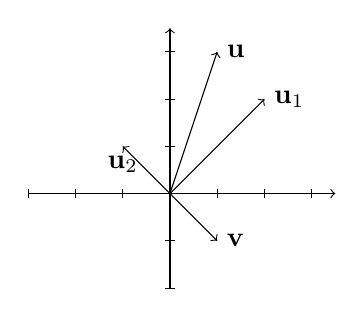
\begin{tikzpicture}[scale=.6]
	\draw[->] (-3,0) -- (3.5,0);
	\draw[->] (0,-2) -- (0,3.5);
	\foreach \x in {-3,-2,-1,1,2,3}
	\draw (\x,.1) -- (\x,-.1);% node[anchor=north] {$\x$};
	\foreach \y in {-2,-1,1,2,3}
	\draw (.1,\y) -- (-.1,\y);% node[anchor=east] {$\y$};
	\draw[->] (0,0) -- (1,3) node[anchor=west] {$\u$};
	\draw[->] (0,0) -- (1,-1) node[anchor=west] {$\v$};
	\draw[->] (0,0) -- (2,2) node[anchor=west] {$\u_1$};
	\draw[->] (0,0) -- (-1,1) node[anchor=north] {$\u_2$};
	\end{tikzpicture}
\end{center}
\end{losning}


\begin{losning}
Vi finner først egenverdiene og egenvektorene til
\[A=
\begin{bmatrix}
4 & 0 & -16 \\
0 & 2 & 0 \\
-3 & 0 & 6
\end{bmatrix}.
\]

\begin{align*}
\det (A-\lambda I) &= \det
\begin{bmatrix}
4-\lambda & 0 & -16 \\
0 & 2-\lambda & 0 \\
-3 & 0 & 6-\lambda
\end{bmatrix}\\
&= (2-\lambda)\det
\begin{bmatrix}
4-\lambda & -16 \\
-3 &  6-\lambda
\end{bmatrix}\\
&=(2-\lambda)((4-\lambda)(6-\lambda)-(-3)(-16))\\
&=(2-\lambda)(\lambda ^2-10\lambda-24)
\end{align*}
Vi ser umiddelbart at $\lambda_1=2$ er en egenverdi. Bruk abc-formelen for å finne resten:
$$\lambda=\frac{-(-10\pm \sqrt{(-10)^2-4(-24)})}{2}=5\pm 7.$$

Dette gir tre egenverdier: $2$,$-2$ og~$12$.

\noindent 
$\lambda=2$:
\begin{align*}
A-2I &=
\begin{bmatrix}
2 & 0 & -16 \\
0 & 0 & 0 \\
-3 & 0 & 4
\end{bmatrix}
\sim
\begin{bmatrix}
1 & 0 & -8 \\
0 & 0 & 0 \\
-3 & 0 & 4
\end{bmatrix}\\
&\sim
\begin{bmatrix}
1 & 0 & -8 \\
-3 & 0 & 4 \\
0 & 0 & 0
\end{bmatrix}
\sim
\begin{bmatrix}
1 & 0 & -8 \\
0 & 0 & -20 \\
0 & 0 & 0
\end{bmatrix}
\end{align*}
Vi ser at $x_2$ er en fri variabel (andre kolonne består kun av null). Videre har vi $-20x_3=0$ slik at $x_3=0$, og $x_1-8x_3=0$ som gir $x_1=0$. Vi kan dermed parametrisere egenrommet til $2$:
$$E_2=\{\vvv{0}{t}{0}|\;\;t\in\mathbb{R}\}=\Sp \vvv{0}{1}{0}.$$ Spesielt er $\vvv{0}{1}{0}$ en egenvektor.

\noindent
Tilsvarende fremgangsmåte for $-2$ og~$12$ gir henholdsvis $\vvv{8}{0}{3}$ og $\vvv{-2}{0}{1}$.


\noindent
Til slutt setter vi inn i formelen for generell løsning:
$$\V{y} = c_1\vvv{0}{1}{0}e^{2t}+c_2\vvv{8}{0}{3}e^{-2t}+c_3 \vvv{-2}{0}{1}e^{12t}.$$
\end{losning}


\begin{losning}
Husk at determinanten ikke endrer seg dersom man legger til et multiplum av en rad til en annen, og determinanten multipliseres med $-1$ dersom man bytter om på to rader:

\begin{align*}
\begin{vmatrix}
3  &  1 - i  & i      & 4      \\
3  &  1      & 1 - 2i & 4 + 7i \\
6i &  2 + 2i & -2     & 3i     \\
-3 & -1 + i  & 1      & 3 - 4i
\end{vmatrix} &=
\begin{vmatrix}
3  &  1 - i   & i      & 4  \\
0  &  i       & 1 - 3i & 7i \\
6i &  2 + 2i  & -2     & 3i \\
-3 & -1 + i   & 1      & 3 - 4i
\end{vmatrix}\\ &=
\begin{vmatrix}
3  &  1 - i  & i      & 4  \\
0  &  i      & 1 - 3i & 7i \\
0  &  0      & 0     & -5i \\
-3 & -1 + i  & 1     & 3 - 4i
\end{vmatrix}\\ &=
\begin{vmatrix}
3 &  1 - i  & i      & 4  \\
0 &  i      & 1 - 3i & 7i \\
0 &  0      & 0      & -5i\\
0 &  0      & 1+i    & 7 - 4i
\end{vmatrix}\\ &=
-\begin{vmatrix}
3 &  1 - i  & i      & 4     \\
0 &  i      & 1 - 3i & 7i    \\
0 &  0      & 1+i    & 7 - 4i\\
0 &  0      & 0      & -5i
\end{vmatrix}.
\end{align*}
Nå kan vi bruke at determinanten til en triangulær matrise er produktet av elementet langs diagonalen:
\[
\begin{vmatrix}
3  &  1 - i  & i      & 4      \\
3  &  1      & 1 - 2i & 4 + 7i \\
6i &  2 + 2i & -2     & 3i     \\
-3 & -1 + i  & 1      & 3 - 4i
\end{vmatrix} 
=-(3)(i)(1+i)(-5i)=-15-15i.
\]

\end{losning}


\begin{losning}
En matrise som tilfredstiller oppgaveteksten kan skrives på formen $A=PDP^{-1}$ hvor
\[
P=\begin{bmatrix}
1  & 1  & 2  & -1 \\
2  & 3  & 4  & -2 \\
0  & 0  & 1  & 3  \\
-3 & -3 & -6 & 4
\end{bmatrix},
\]
og
\[
D=\begin{bmatrix}
1 & 0 & 0  & 0 \\
0 & 1 & 0  & 0 \\
0 & 0 &-1  & 0  \\
0 & 0 & 0  & 3
\end{bmatrix}.
\]

Regn ut
\[
P^{-1}=\begin{bmatrix}
24 & -1 & -2 & 7  \\
-2 & 1  & 0  & 0  \\
-9 & 0  & 1  & -3 \\
3  & 0  & 0  & 1
\end{bmatrix},
\]
og sett inn i $A=PDP^{-1}$:
\[
A=\begin{bmatrix}
34  & 0 & -4 & 11 \\
66  & 1 & -8 & 22 \\
27  & 0 & -1 & 9  \\
-96 & 0 & 12 & -31
\end{bmatrix}.
\]


\end{losning}


\begin{losning}
Radreduser matrisen:

\begin{align*}
\begin{bmatrix}
1 & 5 & 5 \\
2 & 8 & 6 \\
-1 & 3 & 11
\end{bmatrix} &\sim
\begin{bmatrix}
1 & 5 & 5 \\
1 & 4 & 3 \\
-1 & 3 & 11
\end{bmatrix} \sim
\begin{bmatrix}
1 & 5 & 5 \\
0 & -1 & -2 \\
0 & 8 & 16
\end{bmatrix}\\ &\sim
\begin{bmatrix}
1 & 5 & 5 \\
0 & -1 & -2 \\
0 & 1 & 2
\end{bmatrix} \sim
\begin{bmatrix}
1 & 5 & 5 \\
0 & 1 & 2 \\
0 & 0 & 0
\end{bmatrix}.
\end{align*}

Dette viser at vi kun har pivotelement i første og andre kolonne. En basis til kolonnerommet er dermed gitt av 

$$\vvv{1}{2}{-1}, \quad \vvv{5}{8}{3}.$$
Men merk at 
$$\vvv{1}{2}{-1} \boldsymbol{\cdot} \vvv{5}{8}{3} =18. $$
Derfor må vi bruke Gram-Schmidt for å ortogonalisere basisen:
Ta $\V{v}_1=\vvv{1}{2}{-1}$ som første basiselement, og trekk fra den ortogonale projeksjonen ned på denne:
$$\V{v}_2=\vvv{5}{8}{3}-\frac{\V{v}_1 \boldsymbol{\cdot} \vvv{5}{8}{3}}{\V{v}_1 \boldsymbol{\cdot} \V{v}_1} \V{v}_1=\vvv{2}{2}{6}.$$
Vektorene $\V{v}_1$ og~$\V{v}_2$ er en ortogonal basis for kolonnerommet.

% \vvv{1}{2}{-1}, \vvv{2}{2}{6}
\end{losning}


\begin{losning}
Skriv $B$ på elementform:
\[
B=\begin{bmatrix}
b_1 & b_4\\
b_2 & b_5\\
b_3 & b_6
\end{bmatrix}
\]
Produktet $AB$ kan nå uttrykkes ved 
\[
AB=
\begin{bmatrix}
3 & 0 & 4 \\
2 & 1 & 1
\end{bmatrix}
\begin{bmatrix}
b_1 & b_4\\
b_2 & b_5\\
b_3 & b_6
\end{bmatrix}=
\begin{bmatrix}
3b_1+4b_3 & 3b_4+4b_6\\
2b_1+b_2+b_3 & 2b_4+b_5+b_6
\end{bmatrix}
\]

Vi ønsker å bestemme $b_i$-ene slik at $AB=I$;

\[
\begin{bmatrix}
3b_1+4b_3 & 3b_4+4b_6\\
2b_1+b_2+b_3 & 2b_4+b_5+b_6
\end{bmatrix}
=
\begin{bmatrix}
1 & 0\\
0 & 1
\end{bmatrix}.
\]
Dette er fire likninger med seks ukjente

\begin{align*}
3b_1+4b_3&=1\\
2b_1+b_2+b_3&=0\\
3b_4+4b_6&=0\\
2b_4+b_5+b_6&=1.
\end{align*}
%Totalmatrisen er
%\[
%\begin{bmatrix}
%3 & 0 & 4 & 0 & 0 & 0 & 1\\
%2 & 1 & 1 & 0 & 0 & 0 & 0\\
%0 & 0 & 0 & 3 & 0 & 4 & 0\\
%0 & 0 & 0 & 2 & 1 & 1 & 1
%\end{bmatrix}.
%\]
Vi ser at $b_3=t$ og~$b_6=s$ er frie variabler. Multipliser andre og fjerde likning med $3$, og bruk første likning for å eliminere $b_1$ i andre likning; tredje likning for å eliminere $b_4$ i fjerde likning (du kan alternativt skrive opp totalmatrisen til systemet og radredusere):
\begin{align*}
b_1&=\frac{1-4t}{3}\\
b_2&=\frac{5t-2}{3}\\
b_4&=-\frac{4}{3}s\\
b_5&=\frac{5s+3}{3}.
\end{align*}
Alle løsninger kan dermed parametriseres som (du trenger bare å finne en av disse for å svare på oppgaven)

\[\{\begin{bmatrix}
\frac{1-4t}{3} & -\frac{4}{3}s\\
\frac{5t-2}{3} & \frac{5s+3}{3}\\
t & s
\end{bmatrix}|\;\;t,s\in\mathbb{R}\}.
\]

Vi kan for eksempel ta $t$ og~$s$ lik null for å få
\[
B=
\begin{bmatrix}
\frac{1}{3} & 0\\
-\frac{2}{3} & 1\\
0 & 0
\end{bmatrix}.
\]
% f.eks.
%  1/3  0
% -2/3  1
%   0   0
\end{losning}


\begin{losning}
Vi vet at $T(\u)$, $T(\v)$ og~$T(\w)$ er lineært uavhengige, hvor $T$ er en lineærtransformasjon. 

Vi ønsker å vise at $\u$, $\v$ og~$\w$ er lineært uavhengige. Anta at de er lineært avhengige (for å vise at dette umulig kan stemme). Dette betyr -- per definisjon -- at det eksisterer koeffisienter $a$, $b$ og~$c$, ikke alle lik null, slik at
\[
a\u+b\v+c\w=\0. 
\]
Anvend $T$ på begge sider for å få 
\[
T(a\u+b\v+c\w)=T(\0). 
\]
Vi vet at $T$ er lineær som gir
\[
aT(\u)+bT(\v)+cT(\w)=\0. 
\]
Denne likningen betyr i så fall at $T(\u)$, $T(\v)$ og~$T(\w)$ også er lineært avhengige. Men vi \emph{vet} jo at de er lineært uavhengige -- antagelsen er altså umulig . Dermed må $\u$, $\v$ og~$\w$ være lineært uavhengige -- som er det vi ønsket å vise.
\end{losning}
\begin{losning}
Husk at vi skriver $\M_2$ for vektorrommet som består av alle $2 \times 2$-matriser.
La $U$ være mengden av alle symmetriske $2 \times 2$-matriser.
Vis at $U$ er et underrom av~$\M_2$.
Finn en basis for~$U$.  Hva er dimensjonen til~$\M_2$, og hva er dimensjonen til~$U$?
\end{losning}


\begin{losning}
La $A$ være en $m \times n$-matrise med rang~$r$.
Vis at det finnes en $m \times r$-matrise~$B$ og
en $r \times n$-matrise~$C$
slik at $A = BC$.
\end{losning}


\end{document}
